\documentclass[preview]{standalone}
\usepackage{tikz, pgfplots}

\definecolor{pU}{HTML}{003f5c}
\definecolor{pFA}{HTML}{444e86}
\definecolor{pFV}{HTML}{955196}
\definecolor{pCBA}{HTML}{dd5182}
\definecolor{pDP}{HTML}{ff6e54}
\definecolor{pCP}{HTML}{ffa600}

\begin{document}
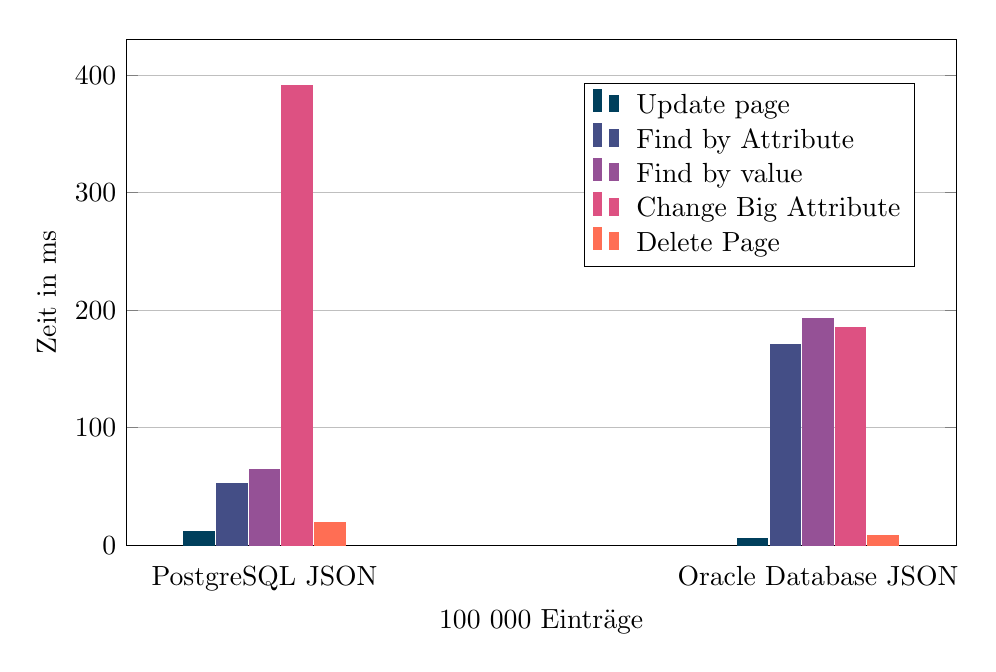
\begin{tikzpicture}
	\begin{axis}[
		width = \textwidth,
		height = 8cm,
		major x tick style = transparent,
		ybar=2*\pgflinewidth,
        bar width=11pt,
        ymajorgrids = true,
        ylabel = {Zeit in ms},
        symbolic x coords={PostgreSQL JSON,Oracle Database JSON},
        xtick = data,
        xlabel style={align=center},
        xlabel = 100 000 Einträge, 
        scaled y ticks = false,
        enlarge x limits=0.25,
        ymin=0,
        legend cell align=left,
                legend style={
                at={(0.95,0.55)},
                anchor=south east,
                column sep=1ex
        }
	]
	
	\addplot[style={pU, fill=pU, mark=none}]
			coordinates {(PostgreSQL JSON, 12)(Oracle Database JSON, 6)};
		
	\addplot[style={pFA, fill=pFA, mark=none}]
			coordinates {(PostgreSQL JSON, 52)(Oracle Database JSON, 171)};
			
	\addplot[style={pFV, fill=pFV, mark=none}]
			coordinates {(PostgreSQL JSON, 64)(Oracle Database JSON, 193)};
	\addplot[style={pCBA, fill=pCBA, mark=none}]
			coordinates {(PostgreSQL JSON, 391)(Oracle Database JSON, 185)};
	\addplot[style={pDP, fill=pDP, mark=none}]
			coordinates {(PostgreSQL JSON, 19)(Oracle Database JSON, 8)};			
	\legend{Update page, Find by Attribute, Find by value, Change Big Attribute, Delete Page}
	\end{axis}
\end{tikzpicture}
\end{document}